\documentclass{article}
\usepackage{algorithm}
\usepackage{algpseudocode}
\usepackage{amsmath}
\usepackage{amssymb}
\usepackage{amsthm}
\usepackage[titletoc]{appendix}
\usepackage{array}
\usepackage[english]{babel}
\usepackage{booktabs}
\usepackage{cancel}
\usepackage{color}
\usepackage{eqparbox}
\usepackage{float}
\usepackage[margin=1in]{geometry}
\usepackage{graphicx}
\usepackage[hidelinks]{hyperref}
% *must* be loaded after hyperref
\usepackage[toc, acronym, numberedsection=nameref]{glossaries}
\usepackage[utf8]{inputenc}
\usepackage{lipsum}
\usepackage{mathtools}
\usepackage[cache=false]{minted}
\usepackage{parskip}
\usepackage{pgfplots}
\usepackage{scalerel}
\usepackage{skull}
\usepackage{subcaption}
\usepackage{titling}
\usepackage{textcomp}
\usepackage{tikz}
\usepackage[compact, explicit]{titlesec}
\usepackage{textcomp}
\usepackage[nottoc]{tocbibind}
\usepackage[textsize=small]{todonotes}
\usepackage[normalem]{ulem}

% Document Settings

\definecolor{__minted_background_color}{rgb}{0.95, 0.95, 0.98}
\definecolor{__minted_highlight_color}{rgb}{0.88, 0.88, 1.0}
\setminted{autogobble=true,
           style=tango,
           breaklines,
           bgcolor=__minted_background_color,
           highlightcolor=__minted_highlight_color,
           mathescape, % Escape math mode everywhere.
           texcomments,  % Enable latex code inside of comments. Useful for referencing equations.
    }

\usetikzlibrary{arrows, automata, shapes, positioning}
\pgfplotsset{compat=1.16}
\numberwithin{equation}{section}
% Sets the width of the margin TODO notes
\setlength{\marginparwidth}{0.84in}
\reversemarginpar{}

% hex #184c9a
\definecolor{__glossary_entry_color}{rgb}{0.094, 0.298, 0.604}
\renewcommand{\glstextformat}[1]{\textbf{\textcolor{__glossary_entry_color}{#1}}}

% Add glos: to the beginning of the glossary labels.
\renewcommand*{\glsautoprefix}{glos:}

% All I want is to have comment italicized, but I cant figure out how
% to properly modify the existing \Comment macro.
% \algrenewcomment[1]{\hfill\eqparbox{COMMENT}{\textit{// #1}}}
\algnewcommand{\IComment}[1]{\Comment{\textit{#1}}}

% TODO: Should this path be relative to the document root or this file?
\graphicspath{{./figures/}}

% Document Definitions

\newcommand{\C}{\mathbb{C}}
\newcommand{\R}{\mathbb{R}}
\newcommand{\Z}{\mathbb{Z}}
\newcommand{\N}{\mathbb{N}}
\renewcommand{\O}{\mathcal{O}}

\theoremstyle{definition}
\newtheorem{defn}{Definition}[section]

\theoremstyle{plain}
\newtheorem{thm}{Theorem}[section]

\renewcommand{\qedsymbol}{$\skull$}

% An inline TODO command. Doesn't play nicely with \todotableofcontents
\newcommand\todoinline[2][]{\todo[inline, caption={TODO}, #1]{
\begin{minipage}{\textwidth-4pt}#2\end{minipage}}}

% Draw clouds around things. Useful in mathematical proofs.
\newcommand{\cloud}[4][\dots]{%
    \raisebox{-0.4\height}{%
        \begin{tikzpicture}
            \node [cloud,
                   draw,
                   cloud puffs=#2,
                   cloud ignores aspect,
                   minimum height=#3,
                   minimum width=#4] {#1};
        \end{tikzpicture}
    }
}

% Use \ceil*{} or \floor*{}
\DeclarePairedDelimiter{\ceil}{\lceil}{\rceil}
\DeclarePairedDelimiter{\floor}{\lfloor}{\rfloor}

\AtBeginDocument{%
\renewcommand{\sectionautorefname}{Problem}
}

% make each \section a problem.
\titleformat{\section}[runin]{\large\bfseries}{}{0pt}{\titlerule[1.5pt]\newline\vspace*{-4pt}
Problem\quad\thesection\newline}[\vspace{0.01ex}{\titlerule[1.5pt]}]


\title{Homework 2}
\author{Austin Gill}
\date{February 15, 2019}

\begin{document}
\maketitle

\section{}
\begin{quote}
    Let $\Sigma = \{a, b\}$ and $L = \{aa, bb\}$. Describe $\overline L$ with set notation.
\end{quote}

\section{}
\begin{quote}
    Find a grammar for the language $L = \{ a^n \mid n \in 2\N \}$
\end{quote}

\section{}
\begin{quote}
    What language does the grammar with these productions generate?
    \begin{align*}
        S & \to Aa \\
        A & \to B  \\
        B & \to Aa
    \end{align*}
\end{quote}

\section{}
\begin{quote}
    Find a regular expression over the alphabet $\{0, 1\}$ to describe all bitstrings without
    leading zeros (except for 0 itself). So the language is the set
    \[ \{0, 1, 10, 11, 100, \dots \} \]
\end{quote}

\section{}\label{prob:5}
\begin{quote}
    Find the quintuple for the DFA in \autoref{fig:5:dfa}.
\end{quote}

\begin{figure}[h]
    \centering
    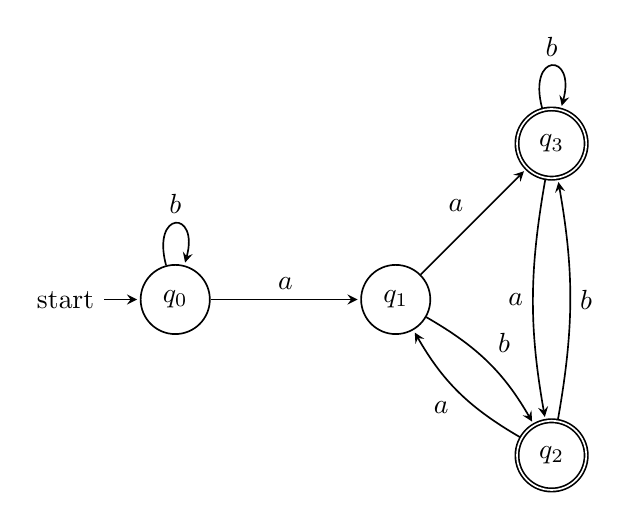
\begin{tikzpicture}[
            ->,
            > = stealth,
            shorten > = 1pt,
            auto,
            node distance = 2.8cm,
            on grid,
            semithick
        ]

        \node[state, initial] (q0) {$q_0$};
        \node[state, right of=q0] (q1) {$q_1$};
        \node[state, accepting, above right of=q1] (q3) {$q_3$};
        \node[state, accepting, below right of=q1] (q2) {$q_2$};

        % \begin{noindent}
        \path (q0) edge[loop above]    node        {$b$} (q0)
                   edge                node        {$a$} (q1)
              (q1) edge                node        {$a$} (q3)
                   edge[bend left=15]  node        {$b$} (q2)
              (q2) edge[bend left=15]  node        {$a$} (q1)
                   edge[bend right=10] node[right] {$b$} (q3)
              (q3) edge[bend right=10] node[left]  {$a$} (q2)
                   edge[loop above]    node        {$b$} (q3);
        % \end{noindent}
    \end{tikzpicture}
    \caption{The DFA for \autoref{prob:5}}\label{fig:5:dfa}
\end{figure}

\section{}
\begin{quote}
    Give a regular expression for the language
    \[L = \{a^n b^m \mid n < 4, m \leq 4\} \]
\end{quote}

\section{}
\begin{quote}
    Describe the language for the regular expressions
    \begin{enumerate}
        \item $a + b$
        \item $a + b^*$
        \item $ab^* + bc^*$
    \end{enumerate}
    Construct an NFA for the regular expression
    \[r = {(a + b)}^*\]
\end{quote}

\end{document}
